\documentclass[a4paper,12pt]{extarticle}
\usepackage[T2A]{fontenc}
\usepackage[utf8]{inputenc}
\usepackage[russian]{babel}
\usepackage{amsmath, amssymb}
\usepackage{graphicx}
\usepackage{geometry}
\usepackage{caption}
\usepackage{float}

% Настройка полей для стандартного отчёта
\geometry{left=2cm, right=2cm, top=2cm, bottom=2cm}

% \title{\textbf{Теоретическая часть}\\ Лабораторная работа №120:\\ Когерентность света}
% \author{}
% \date{}

\begin{document}

% \maketitle

\title{\begin{center}Лабораторная работа №4.2.5:\end{center}
Когерентность света}
\author{Струков О. И. \\ Б04-404}
\date{}

\thispagestyle{empty}
\pagenumbering{gobble}
\maketitle
\newpage
\pagenumbering{arabic}


\section*{Теоретическая часть}

% Понятие \textbf{когерентности} (от лат. \textit{cohaerens} -- находящийся в связи) возникло в оптике как характеристика, определяющая способность света к интерференции. Интерференция описывает взаимное усиление или ослабление световых волн при их наложении друг на друга. Обычные тепловые или газоразрядные источники света являются генераторами случайных полей, поэтому возникает проблема описания взаимной согласованности (зависимости, корреляции) световых колебаний в разных точках пространства в различные моменты времени.

% В данной работе рассматривается частный случай, в котором исследуется согласованность колебаний в двух точках с координатами $\mathbf{r}_1$ и $\mathbf{r}_2$ в моменты времени $t_1$ и $t_2$. Световые колебания считаются квазимонохроматическими с центральной частотой $\omega_0$. Поле считается скалярным, то есть не учитываются эффекты, связанные с поляризацией излучения. Если ввести комплексную амплитуду световой волны $A(\mathbf{r}, t)$, то поле в точке $\mathbf{r}$ в момент времени $t$ удобно записать в виде $A(\mathbf{r}, t)e^{i\omega_0 t}$, причём амплитуда $A(\mathbf{r}, t)$ мало меняется за период световых колебаний $2\pi/\omega_0 \approx 10^{-15}$ с.

\qquad\textbf{Цель работы:} оценка длины волны излучения полупроводникового лазера, определение зависимости радиуса когерентности от размера источника, оценка спектрального диапазона чувствительности зрительной системы экспериментатора.

\textbf{В работе используются:} лазер, лампы накаливания с блоком питания, объектив, оптические щели, микроскоп.

\subsection*{Функция когерентности и видность интерференционной картины}

За меру когерентности световых полей в точках $\mathbf{r}_1$ и $\mathbf{r}_2$ в моменты времени $t_1$ и $t_2$ выбирают нормированное среднее произведение амплитуд полей:
\begin{equation}
\gamma = \frac{\langle A(\mathbf{r}_1,t_1)e^{i\omega_0 t_1} \cdot A^*(\mathbf{r}_2,t_2)e^{-i\omega_0 t_2} \rangle}{\sqrt{\langle|A(\mathbf{r}_1,t_1)|^2\rangle \cdot \langle|A(\mathbf{r}_2,t_2)|^2\rangle}}.
\label{eq:gamma_def}
\end{equation}
Черта в формуле (\ref{eq:gamma_def}) обозначает статистическое усреднение или усреднение по времени. В данной работе выбирается усреднение по времени, так как поле стационарное (статистические характеристики поля не зависят от времени), а время регистрации интенсивностей полей (глазом или видеокамерой) много больше периода колебаний световых волн.

Если случайное световое поле является однородным в пространстве и его статистические характеристики не зависят от времени, то функция когерентности $\gamma$ не зависит от координат $\mathbf{r}_1$, $\mathbf{r}_2$ и моментов времени $t_1$ и $t_2$, а зависит только от их разности $\rho = |\mathbf{r}_2 - \mathbf{r}_1|$ и $\tau = t_2 - t_1$ (время задержки). Входящая в (\ref{eq:gamma_def}) величина $|A(\mathbf{r}, t)|^2$ пропорциональна интенсивности света. Для выбранной пары точек интенсивность света будем считать постоянной и обозначим её через $|A|^2$. В приведённом приближении комплексную функцию когерентности можно записать в виде:
\begin{equation}
\gamma(\rho,\tau)= e^{-i\omega_0\tau} \frac{\langle A(\mathbf{r},t)A^*(\mathbf{r}+\mathbf{\rho},t+\tau) \rangle}{|A|^2}.
\label{eq:gamma_simplified}
\end{equation}
В предельном случае, когда точки близки друг к другу и время задержки мало, $|\gamma(0,0)| = 1$. Если $|\gamma(\rho,\tau)| = 1$, то говорят о полной когерентности колебаний. При $0 < |\gamma(\rho,\tau)| < 1$ свет считается частично когерентным.

Найдём связь между функцией когерентности и измеряемой в оптике характеристикой, называемой \textbf{видностью} (контрастностью). Пусть оптическая система позволяет наложить друг на друга поля $A(\mathbf{r}, t)e^{i\omega_0 t}$ и $A(\mathbf{r}+\mathbf{\rho},t+\tau)e^{i\omega_0(t+\tau)}$ и измерить интенсивность суммарного поля. Используя (\ref{eq:gamma_simplified}), получаем интенсивность:
\begin{equation}
I \approx 2|A|^2 \left[1 + |\gamma(\rho,\tau)| \cos(\omega_0 \tau - \delta(\rho,\tau))\right],
\label{eq:intensity}
\end{equation}
где $\delta(\rho,\tau)$ -- фаза комплексной функции когерентности. Зафиксируем расстояние между точками $\rho$ и учтём, что при небольших изменениях времени задержки $\tau$ фаза $\delta$ меняется пренебрежимо мало по сравнению с $\omega_0\tau$. Тогда в максимуме суммарного поля (интерференционной картины) интенсивность равна $I_{max} \approx 1 + |\gamma(\rho,\tau)|$, а в минимуме $I_{min} \approx 1 - |\gamma(\rho,\tau)|$.

Используя определение видности (контрастности) $V$, получим:
\begin{equation}
V(\rho,\tau)= \frac{I_{max} - I_{min}}{I_{max} + I_{min}} = |\gamma(\rho,\tau)|.
\label{eq:visibility}
\end{equation}
Для некогерентных полей $V = 0$, то есть имеет место равномерная засветка. Глаз различает интерференционную картину при $V > 0,1$.

\begin{figure}[H]
    \centering
    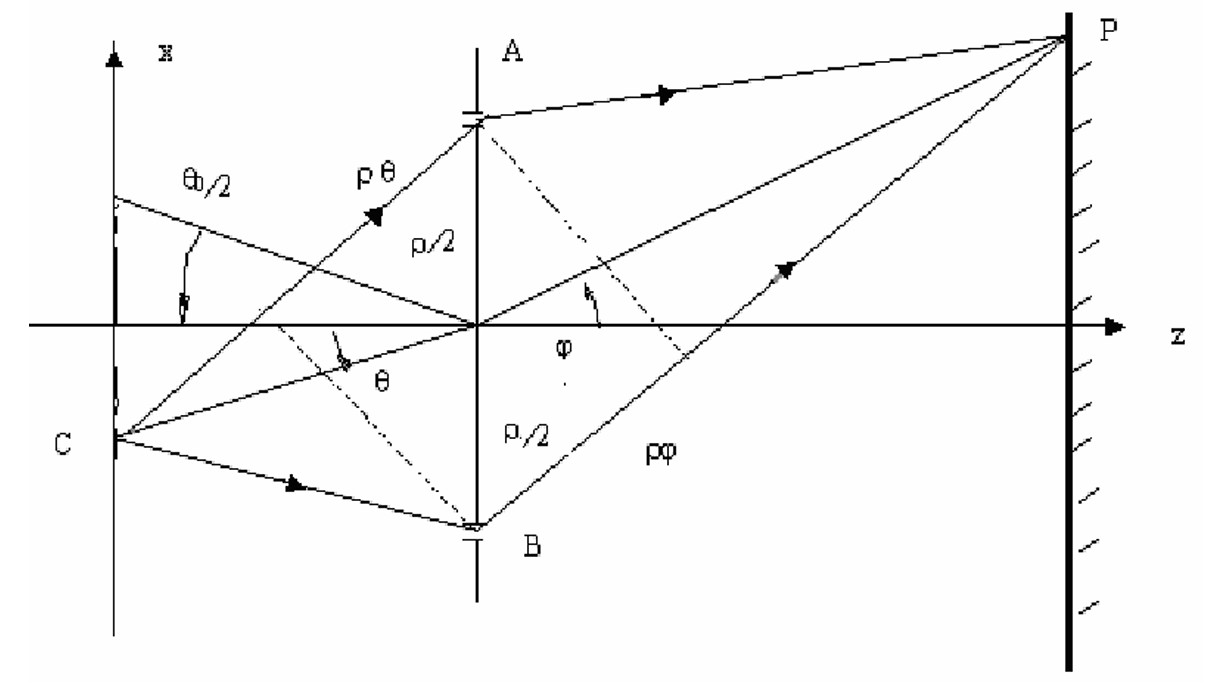
\includegraphics[width=0.6\textwidth]{fig1_scheme.jpg}
    \caption{Принципиальная схема для измерения функции когерентности.}
    \label{fig:scheme}
\end{figure}

\subsection*{Временная когерентность и ширина спектра}

Рассмотрим упрощённую задачу вычисления контрастности интерференционной картины. Пусть нас интересует когерентность в точках $A$ и $B$, а поле распространяется в положительном направлении оси $z$ (рис. \ref{fig:scheme}). Расстояние между точками $AB = \rho$ мы зафиксировали. Для реализации времени задержки $\tau$ воспользуемся идеей Т. Юнга. Поместим в плоскость, перпендикулярную оси $z$, непрозрачный очень тонкий экран с небольшими отверстиями около этих точек.

Регистрируемый спектр оптического поля зависит как от спектра источника (галогенная лампа, полупроводниковый лазер), так и от спектральной чувствительности приёмника. Форму регистрируемого спектра удобно описывать гауссовой кривой. Будем считать, что в интервале частот $\omega$ и $\omega + d\omega$ интенсивность света равна:
\begin{equation}
dI = \frac{I_1}{\sqrt{\pi}\Omega} e^{-\frac{(\omega-\omega_0)^2}{\Omega^2}} d\omega,
\end{equation}
где $\omega_0$ -- центральная частота, $\Omega$ -- ширина спектра излучения, $I_1$ -- полная интенсивность излучения источника во всем спектральном интервале.

Интенсивность света в точке наблюдения $P$ с учётом спектрального распределения определяется интегралом:
\begin{equation}
I_P = I_0 \left[ 1 + \cos\left(\frac{\rho\omega_0}{c}(\varphi - \theta)\right) e^{-\left[\frac{\rho \Omega}{2c}(\varphi-\theta)\right]^2} \right],
\label{eq:intensity_spectrum}
\end{equation}
где $I_0$ -- константа, $\varphi$ -- угол дифракции, $\theta$ -- угол, под которым виден источник. Зависимость интенсивности света от угла дифракции имеет вид интерференционных полос с меняющейся контрастностью (см. рис. \ref{fig:intensity_plot}).

\begin{figure}[H]
    \centering
    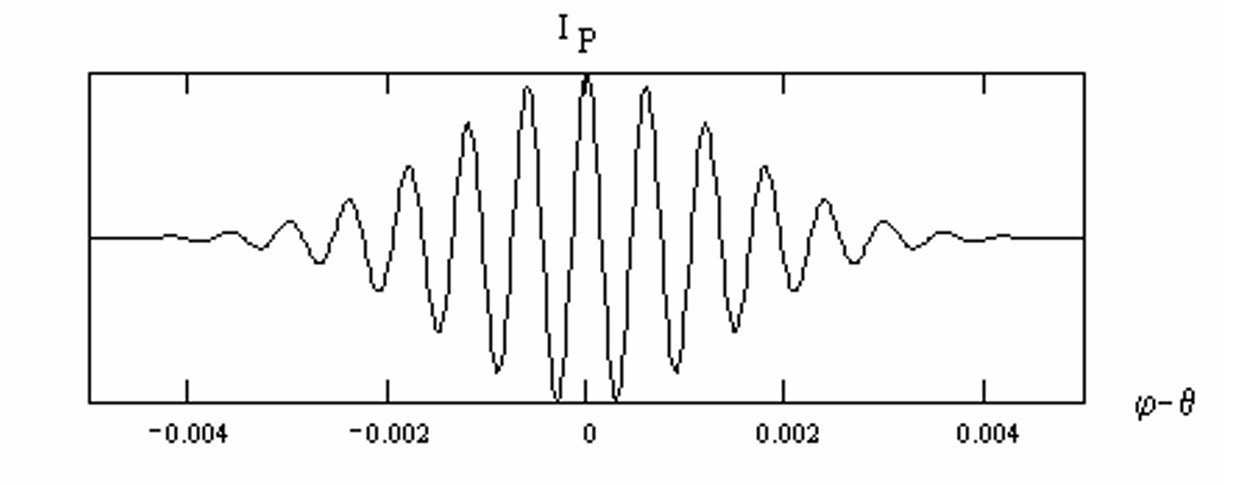
\includegraphics[width=0.6\textwidth]{fig2_intensity.jpg}
    \caption{Зависимость интенсивности света от угла дифракции.}
    \label{fig:intensity_plot}
\end{figure}

Огибающая интерференционных полос вида $e^{-\left[\frac{\rho \Omega}{2c}(\varphi-\theta)\right]^2}$ имеет смысл контрастности интерференционной картины. Введём рабочее определение величины времени и длины когерентности. На опыте можно определить наибольший номер максимума интерференционной полосы $m_{\text{ког}}$, которая находится на пределе разрешения глазом. Будем считать, что этот предел равен среднему для глаза $V_0 = 0,1$. Для этого определения максимальная разность хода, при которой наблюдается интерференция, или \textbf{длина когерентности}:
\begin{equation}
\Delta_{\text{ког}} = m_{\text{ког}} \lambda_0,
\label{eq:coh_length}
\end{equation}
и \textbf{время когерентности} или максимальная задержка:
\begin{equation}
\tau_{\text{ког}} = \frac{\Delta_{\text{ког}}}{c} \approx \frac{2\pi m_{\text{ког}}}{\omega_0}.
\label{eq:coh_time}
\end{equation}
Зная величину $m_{\text{ког}}$, можно оценить ширину спектра источника излучения. Длина когерентности связана с шириной спектра источника соотношением:
\begin{equation}
\Delta_{\text{ког}} = \frac{\lambda_0^2}{\Delta\lambda},
\end{equation}
где $\Delta\lambda$ -- полная ширина спектра в длинах волн. Для широкополосных источников (лампа накаливания) длина когерентности мала (порядка 1 мкм), что требует жёстких условий на разность хода интерферирующих волн.

\subsection*{Пространственная когерентность и протяжённый источник}

Пусть источником излучения является не точка, а тонкая нить, расположенная вдоль оси $x$. Угловой размер нити равен $\theta_0$, нить будем считать абсолютно некогерентным источником света. Для нахождения интенсивности света в точке наблюдения следует просуммировать распределение интенсивности (\ref{eq:intensity_spectrum}) по всем излучающим элементам нити.

Переход к протяжённому источнику уменьшает контрастность изображения в плоскости наблюдения, поэтому угловой размер нити $\theta_0$ должен быть малым. Контрастность интерференционной картины уменьшается не только с увеличением времени задержки, что связано с шириной спектра источника $\Omega$, но и с увеличением расстояния между точками $\rho$, что определяется конечным угловым расстоянием нити $\theta_0$. Контрастность обращается в ноль, если расстояние между отверстиями равно \textbf{радиусу поперечной когерентности}:
\begin{equation}
\rho_{\text{ког}} = \frac{\lambda_0}{\theta_0}.
\label{eq:transverse_coh}
\end{equation}
Для расстояния, равного $\rho_{\text{ког}}$, интенсивность света в плоскости наблюдения постоянна.

Для протяжённого одномерного источника интенсивность света в точке наблюдения описывается выражением:
\begin{equation}
I_p = I_0 \left\{ 1 + e^{-\left(\frac{\rho\Omega}{2c}\varphi\right)^2} \cdot \frac{\sin\left(\frac{\rho\omega_0\theta_0}{2c}\right)}{\frac{\rho\omega_0\theta_0}{2c}} \cdot \cos\left(\frac{\rho\omega_0}{c}\varphi\right) \right\}.
\label{eq:extended_source}
\end{equation}
Используя (\ref{eq:extended_source}), приведём выражение для функции когерентности в её собственных переменных: время задержки $\tau$ и расстояние между точками на плоскости (источник света -- нить):
\begin{equation}
|\gamma(\rho,\tau)| = V(\rho,\tau) = e^{-\left(\frac{\Omega \tau}{2}\right)^2} \left| \frac{\sin\left(\frac{\pi\theta_0}{\lambda_0}\rho\right)}{\frac{\pi\theta_0}{\lambda_0}\rho} \right|.
\label{eq:gamma_final}
\end{equation}

\begin{figure}[H]
    \centering
    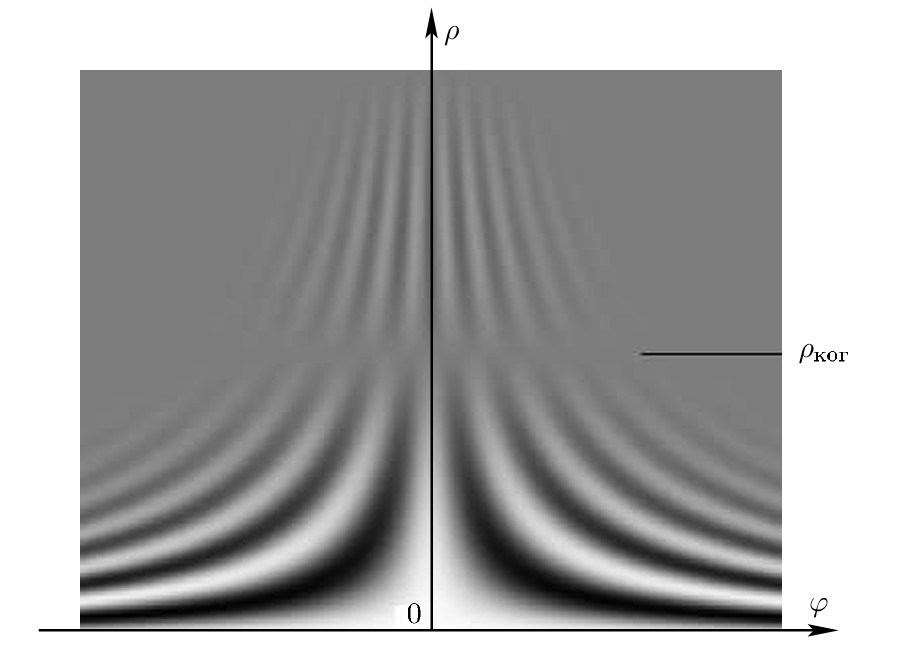
\includegraphics[width=0.6\textwidth]{fig3_3d.jpg}
    \caption{Интенсивность в плоскости наблюдения для протяжённого источника.}
    \label{fig:3d_plot}
\end{figure}

\subsection*{Описание интерферометра}

В работе используется интерферометр, специально сконструированный для визуального наблюдения распределения интенсивности (\ref{eq:extended_source}). Экран с отверстиями помещается в плоскости $(x,y)$, плоскость $(x_1,y_1)$ -- плоскость наблюдения, $z$ -- оптическая ось системы.

В нашем интерферометре используются щели в виде креста. Ширина щелей меняется от 70 до 100 мкм. Для пространственного разделения дифракционных картин от пар отверстий помещаются цилиндрические линзы. Окончательное распределение интенсивности света в плоскости наблюдения интерферометра возникает, если в экране расположить много пар отверстий вдоль биссектрис координатных углов или изготовить экран в виде двух взаимно перпендикулярных узких щелей.

Приведём формулы пересчёта координат $x_1, y_1$ в переменные $\varphi$ и $\rho$, входящие в (\ref{eq:extended_source}):
\begin{equation}
\varphi = \frac{x_1}{b}; \quad \rho = \frac{2a}{b}|y_1|,
\label{eq:coords_transform}
\end{equation}
где $a$ -- расстояние от экрана до объектива, $b$ -- фокусное расстояние объектива.

\begin{figure}[H]
    \centering
    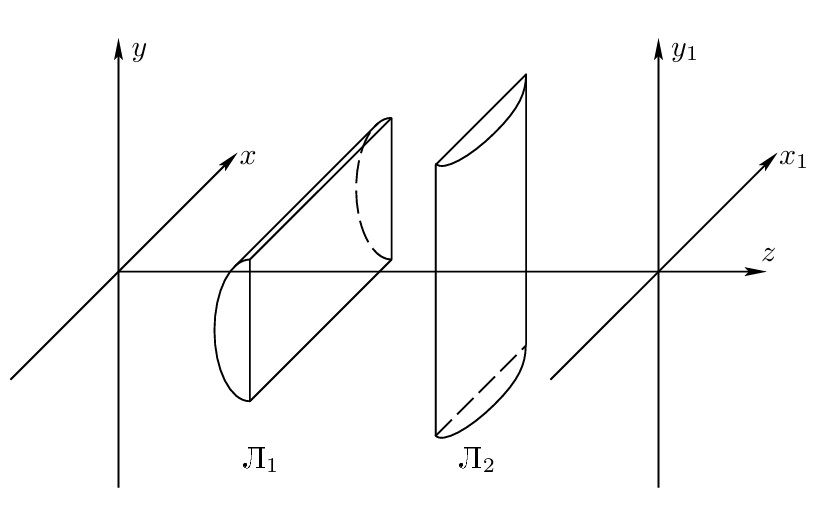
\includegraphics[width=0.6\textwidth]{fig4_interferometer.jpg}
    \caption{Принципиальная схема интерферометра.}
    \label{fig:interferometer}
\end{figure}

% \section*{Заключение}

% Таким образом, когерентность света характеризуется функцией когерентности $\gamma(\rho,\tau)$, модуль которой равен видимости интерференционной картины. Различают временную когерентность (связана с шириной спектра источника) и пространственную (поперечную) когерентность (связана с угловым размером источника). Длина когерентности обратно пропорциональна ширине спектра, а радиус поперечной когерентности обратно пропорционален угловому размеру источника. Для наблюдения интерференции необходимо выполнение условий: разность хода $\le$ длина когерентности, расстояние между точками $\le$ радиус поперечной когерентности. В данной лабораторной работе эти параметры измеряются с помощью специально настроенного интерферометра с использованием как лазерного излучения, так и излучения галогенной лампы.




\section*{Ход работы}

\subsection*{Определение средней длины волны света источника}

\qquad При выполнении работы была собрана установка по схеме в описании, расстояние между линзой и микроскопом 42 см, между линзой и тонкой крестовой щелью (или проволокой для калибровки) 37 см, между перекрестием и щелью возле источника 90,5 см.

Была проведена калибровка шкалы в микроскопе с помощью проволоки диаметром 1 мм. Цена деления соответствует 0,67 мм.

\begin{figure}[H]
    \centering
    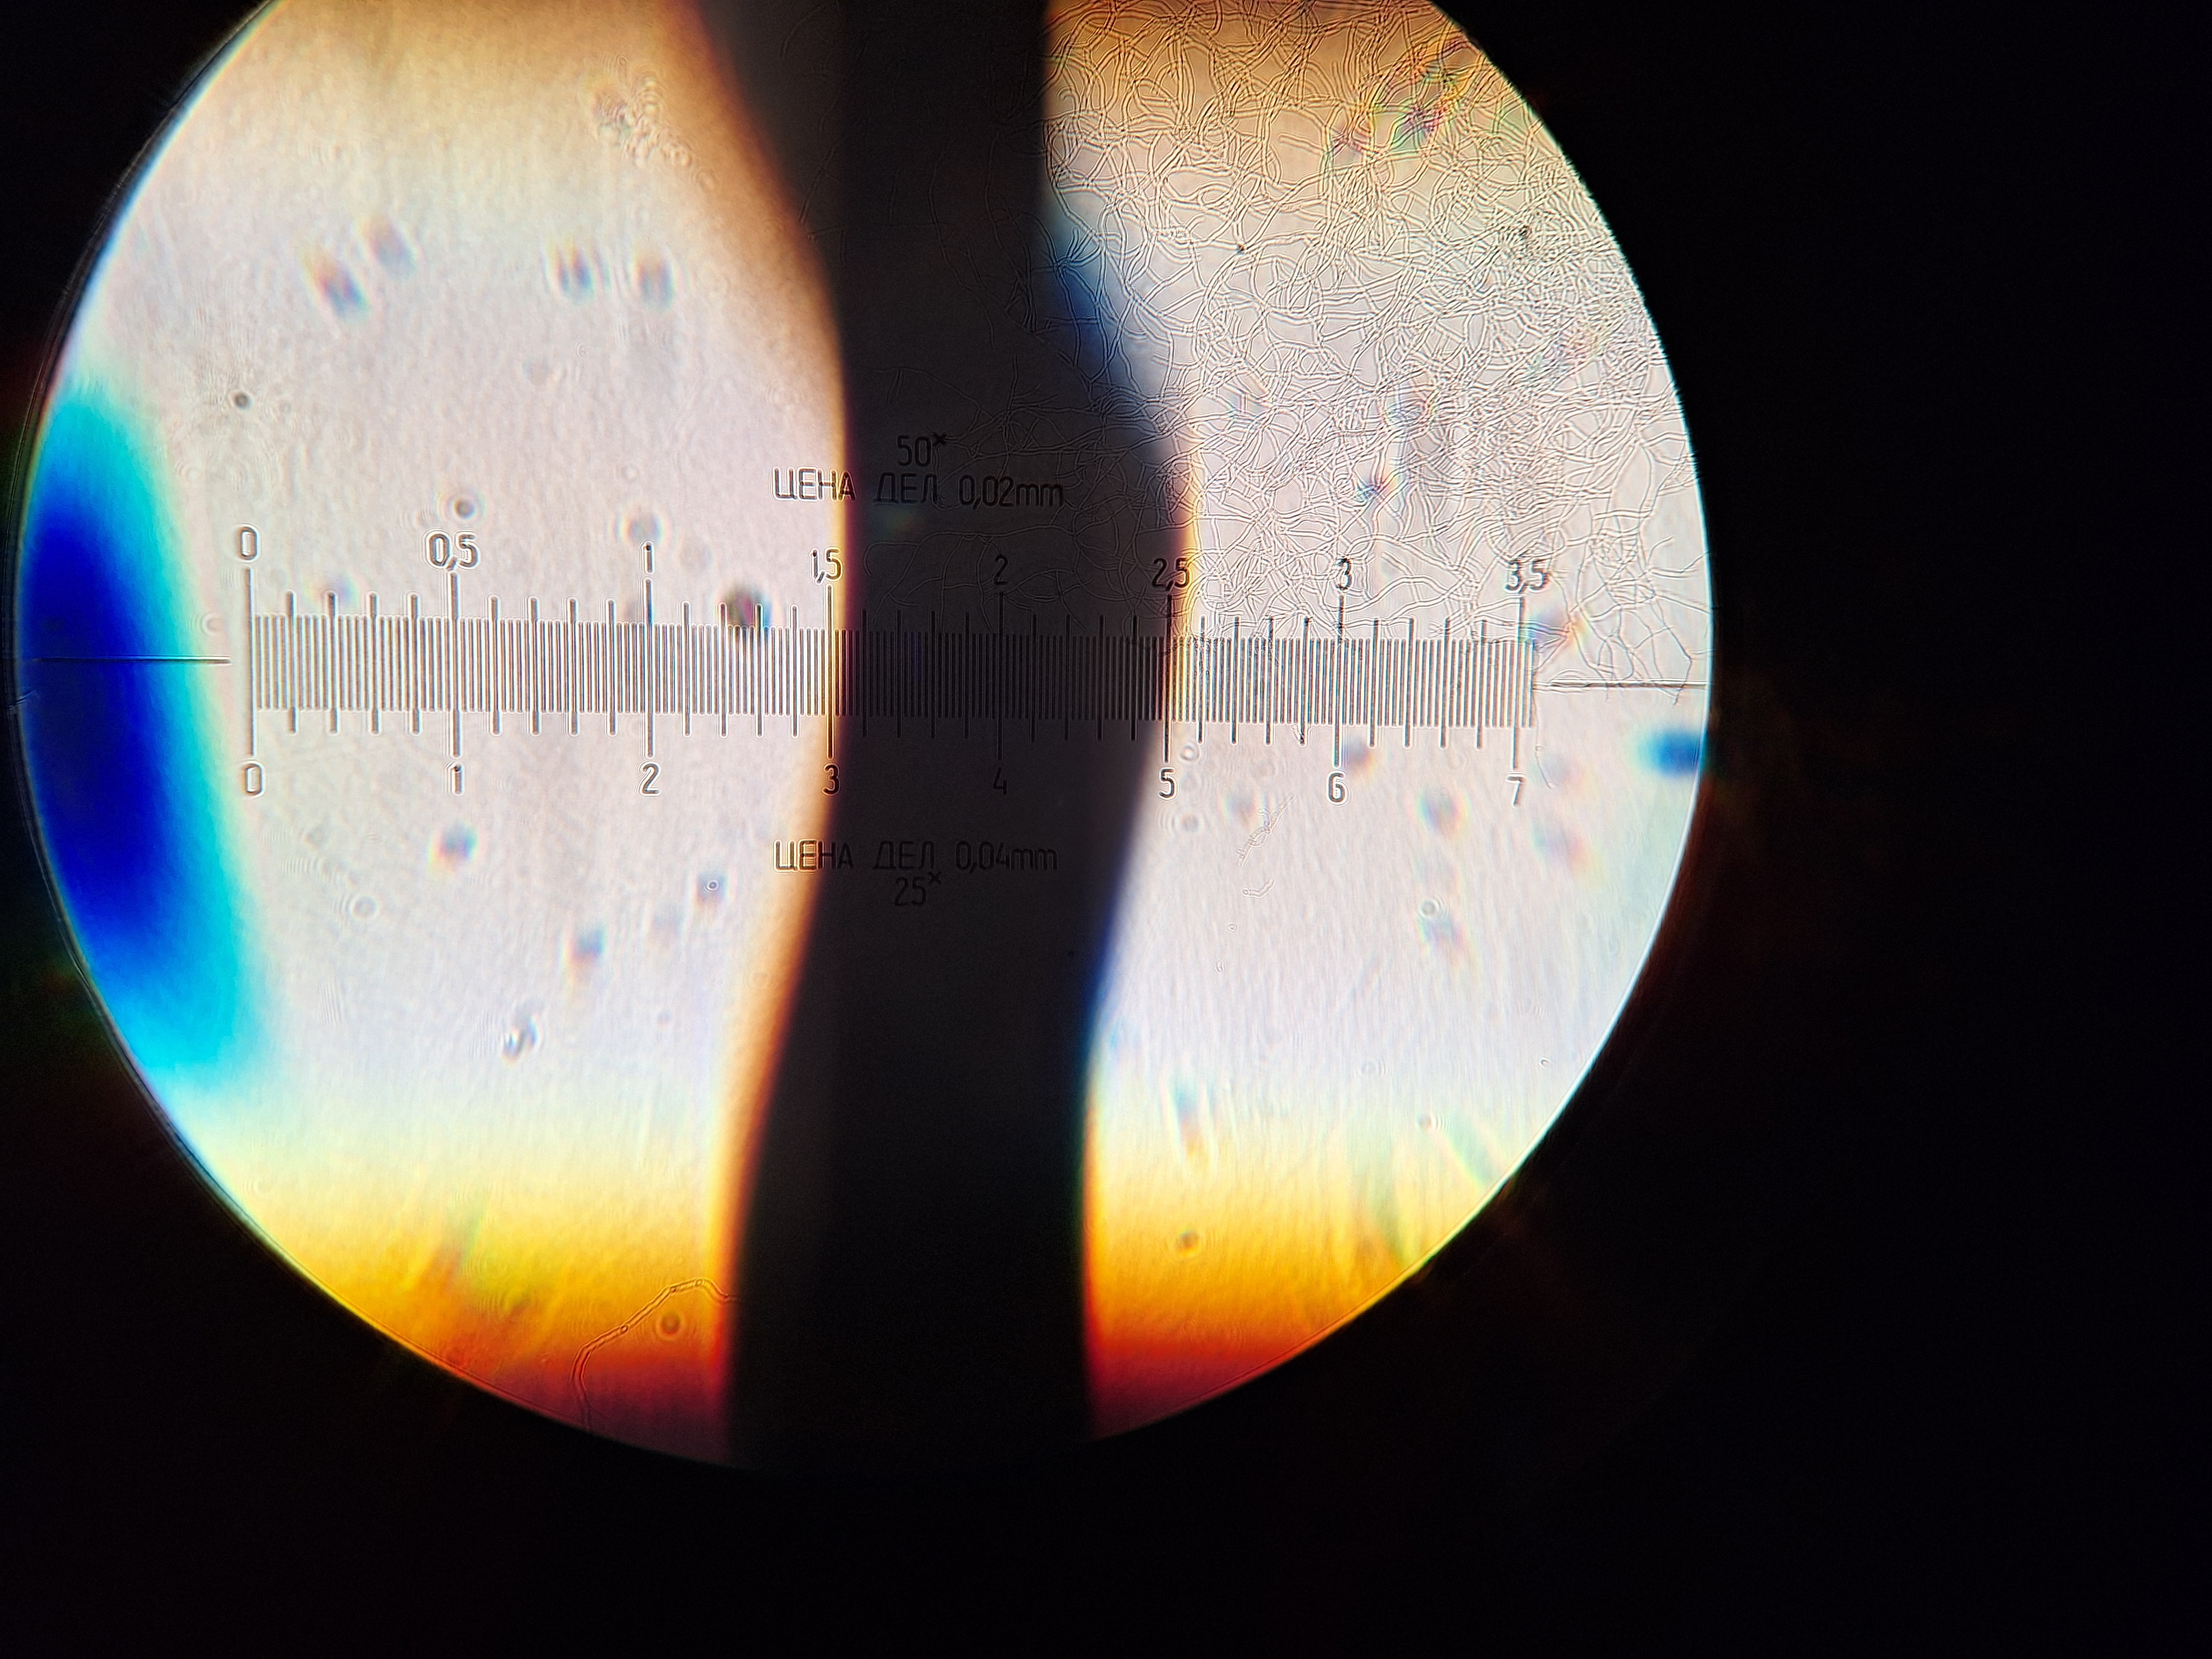
\includegraphics[width=0.6\textwidth]{20260319_101455.jpg}
    \caption{Фото проволоки для калибровки шкалы}
\end{figure}

После установки перекрестия на место проволоки и настройки системы в микроскоп стала видна интерференционная картина (рис. 6), после чего была снята зависимость радиуса когерентности от соответствующей ширины щели. Её график изображён на рисунке 7.

\begin{figure}[H]
    \centering
    
\includegraphics[width=0.6\textwidth]{1.jpg}
    \caption{Интерференционная картина, видимая в микроскоп}
\end{figure}

\begin{figure}[H]
    \centering
    \includegraphics[width=0.8\textwidth]{Точки.pdf}
    \caption{График зависимости радиуса когерентности от ширины щели}
\end{figure}


Поскольку радиус когерентности $\rho = \dfrac{\lambda_0 L}{d}$, где $\lambda_0$ -- средняя длина волны света лампы, $L = 90,5$ см -- расстояние от входной щели до щелей интерферометра, $d$ -- ширина входной щели, то из коэффициента наклона прямой линейного участка зависимости $\rho\left(\dfrac{1}{d}\right)$ можно найти $\lambda_0$.


\begin{figure}[H]
    \centering
    \includegraphics[width=0.8\textwidth]{Прямая.pdf}
    \caption{График зависимости $\rho\left(\dfrac{1}{d}\right)$}
\end{figure}

Коэффициент наклона $k = 0,4185$ мм$^2$, отсюда $\lambda_0 = k/L \approx 462$ нм


\subsection*{Определение длины и времени когерентности и ширины спектра}

По формуле $\Delta = m \lambda_{max}$, где максимальный порядок интерференции $m = 13$ (при ширине щели 0,1 мм),
а $\lambda_{max} = 560$ нм -- длина волны для максимальной чувствительности, была определена длина когерентности $\Delta = 7280$ нм.
Отсюда время когерентности $\tau = \Delta/c \approx 2,43 \cdot 10^{-14}$ с
и ширина спектра $\Delta \lambda = \lambda_{max}/m \approx 43,08$ нм.

Для измеренного значения длины волны $\lambda_0 = 462$ нм эти величины составляют $\Delta_0 = 6006$ нм, $\tau_0 = 2,00 \cdot 10^{-14}$ с, $\Delta \lambda_0 = 35,54$ нм.






\section*{Вывод}
\qquad В резултате выполнения работы была определна средняя длина волны света лампы, составившая 462 нм, что достаточно близко к ожидаемому значению порядка 560 нм, а также рассчитаны длина и время когерентности и ширина спектра, которые тоже близки к ожидаемым значениям.






\end{document}